% Topic extraction pipeline (Stage 3) — schematic for the paper.
% Two tracks extracted independently from different layers of the record
% (hearing summaries vs. member turns); Track 1 induces the codebook through
% consensus clustering and researcher ratification; Track 2's stance records
% are assigned INTO the frozen codebook. CAP is post-hoc gold only — the red
% firewall notes mark what is guaranteed never to enter the pipeline.
% All numbers measured in scripts/python/03_topic_extraction/ (final chain).
% Compile: xelatex fig_topic_extraction.tex
\documentclass[tikz]{standalone}
\usetikzlibrary{positioning,calc,arrows.meta}

% Project palette: Royal Navy (data/flow), Deep Academic Red (firewalls /
% guarantees), Muted Royal Green (stage outputs). Tints stay in family.
\definecolor{navy}{HTML}{003049}
\definecolor{navylight}{HTML}{E8EEF2}
\definecolor{red1}{HTML}{A30006}
\definecolor{green1}{HTML}{7C9885}
\definecolor{greenlight}{HTML}{EDF2EF}
\definecolor{ink}{HTML}{2B2B2B}

\begin{document}
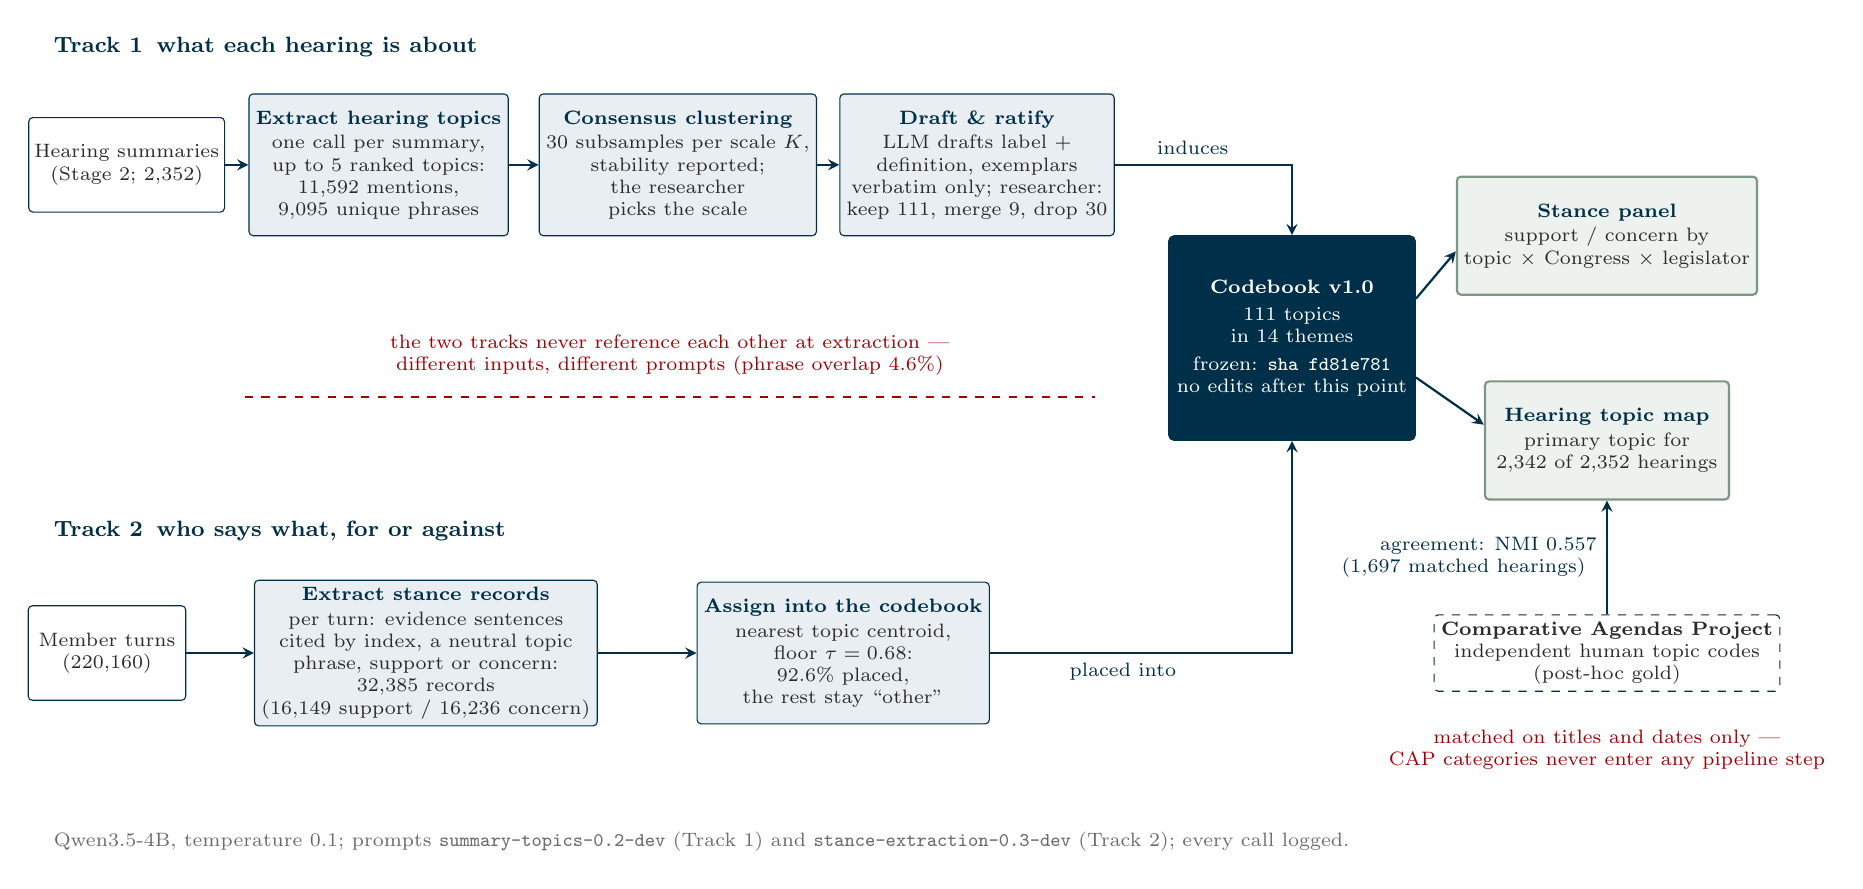
\begin{tikzpicture}[
  font=\footnotesize,
  every node/.style={text=ink},
  raillabel/.style={font=\footnotesize\bfseries, text=navy, anchor=west},
  box/.style={draw=navy, fill=navylight, rounded corners=1.5pt, align=center,
              minimum width=30mm, minimum height=18mm, inner sep=2.5pt,
              font=\scriptsize},
  inbox/.style={draw=navy, fill=white, rounded corners=1.5pt, align=center,
                minimum width=20mm, minimum height=12mm, inner sep=2pt,
                font=\scriptsize},
  outbox/.style={draw=green1, thick, fill=greenlight, rounded corners=1.5pt,
                 align=center, minimum width=31mm, minimum height=15mm,
                 inner sep=2.5pt, font=\scriptsize},
  capbox/.style={draw=navy, dashed, fill=white, rounded corners=1.5pt,
                 align=center, inner sep=2.5pt, font=\scriptsize},
  fw/.style={font=\scriptsize, text=red1, align=center},
  note/.style={font=\scriptsize, text=ink!70, align=center},
  flow/.style={-{stealth}, navy, thick},
]

% ======================================================= Track 1 (top rail)
\node[raillabel] at (-1.95,5.0) {Track 1\enspace what each hearing is about};

\node[inbox] (in1) at (-0.9,3.5) {Hearing summaries\\(Stage 2; 2{,}352)};

\node[box] (t1a) at (2.3,3.5)
  {\textbf{\textcolor{navy}{Extract hearing topics}}\\[1pt]
   one call per summary,\\up to 5 ranked topics:\\11{,}592 mentions,\\9{,}095 unique phrases};
\node[box] (t1b) at (6.1,3.5)
  {\textbf{\textcolor{navy}{Consensus clustering}}\\[1pt]
   30 subsamples per scale $K$,\\stability reported;\\the researcher\\picks the scale};
\node[box] (t1c) at (9.9,3.5)
  {\textbf{\textcolor{navy}{Draft \& ratify}}\\[1pt]
   LLM drafts label +\\definition, exemplars\\verbatim only; researcher:\\keep 111, merge 9, drop 30};

\draw[flow] (in1.east) -- (t1a.west);
\draw[flow] (t1a.east) -- (t1b.west);
\draw[flow] (t1b.east) -- (t1c.west);

% ======================================================= the frozen codebook
\node[draw=navy, fill=navy, rounded corners=2pt, align=center,
      minimum width=29mm, minimum height=26mm, inner sep=3pt,
      font=\scriptsize] (cb) at (13.9,1.3)
  {\textcolor{white}{\textbf{Codebook v1.0}}\\[2pt]
   \textcolor{white}{111 topics}\\
   \textcolor{white}{in 14 themes}\\[2pt]
   \textcolor{white}{frozen: \texttt{sha fd81e781}}\\
   \textcolor{white}{no edits after this point}};

\draw[flow] (t1c.east) -| (cb.north)
  node[pos=0.22, above, font=\scriptsize, text=navy] {induces};

% ======================================================= Track 2 (bottom rail)
\node[raillabel] at (-1.95,-1.15) {Track 2\enspace who says what, for or against};

\node[inbox] (in2) at (-1.15,-2.7) {Member turns\\(220{,}160)};

\node[box] (t2a) at (2.9,-2.7)
  {\textbf{\textcolor{navy}{Extract stance records}}\\[1pt]
   per turn: evidence sentences\\cited by index, a neutral topic\\
   phrase, support or concern:\\32{,}385 records\\
   (16{,}149 support / 16{,}236 concern)};
\node[box] (t2b) at (8.2,-2.7)
  {\textbf{\textcolor{navy}{Assign into the codebook}}\\[1pt]
   nearest topic centroid,\\floor $\tau=0.68$:\\92.6\% placed,\\the rest stay ``other''};

\draw[flow] (in2.east) -- (t2a.west);
\draw[flow] (t2a.east) -- (t2b.west);
\draw[flow] (t2b.east) -| (cb.south)
  node[pos=0.22, below, font=\scriptsize, text=navy] {placed into};

% ============================================= independence firewall (red)
\draw[red1, dashed, thick] (0.6,0.55) -- (11.4,0.55);
\node[fw, anchor=south] at (6.0,0.7)
  {the two tracks never reference each other at extraction ---\\
   different inputs, different prompts (phrase overlap 4.6\%)};

% ======================================================= outputs
\node[outbox] (ostance) at (17.9,2.6)
  {\textbf{\textcolor{navy}{Stance panel}}\\[1pt]
   support / concern by\\topic $\times$ Congress $\times$ legislator};
\node[outbox] (omap) at (17.9,0.0)
  {\textbf{\textcolor{navy}{Hearing topic map}}\\[1pt]
   primary topic for\\2{,}342 of 2{,}352 hearings};

\draw[flow] ($(cb.east)+(0,0.5)$) -- ($(ostance.west)+(0,-0.2)$);
\draw[flow] ($(cb.east)+(0,-0.5)$) -- ($(omap.west)+(0,0.2)$);

% ======================================================= CAP validation
\node[capbox] (cap) at (17.9,-2.7)
  {\textbf{Comparative Agendas Project}\\
   independent human topic codes\\(post-hoc gold)};
\draw[flow] (cap.north) -- (omap.south)
  node[midway, left, font=\scriptsize, text=navy, align=right]
  {agreement: NMI 0.557\\(1{,}697 matched hearings)\enspace};
\node[fw, anchor=north] at (17.9,-3.55)
  {matched on titles and dates only ---\\
   CAP categories never enter any pipeline step};

% ======================================================= footer
\node[note, anchor=north west, align=left] at (-1.95,-4.85)
  {Qwen3.5-4B, temperature 0.1; prompts \texttt{summary-topics-0.2-dev} (Track 1) and
   \texttt{stance-extraction-0.3-dev} (Track 2); every call logged.};

\end{tikzpicture}
\end{document}
